\documentclass{MathNoteCN}

\emergencystretch=3em
\hypersetup{hidelinks}

\title{DeepSeek-V4 技术解读\\ 从 V1 到 V4 的架构演进与百万上下文效率}
\author{VideoNote}
\date{2026 年 8 月 4 日}

\begin{document}
\maketitle

\begin{note}
\textbf{一句话结论}:DeepSeek-V4 不是"更大",而是把注意力从 $O(n^2)$ 的计算复杂度里解放出来,用 \textbf{CSA+HCA 混合注意力}、\textbf{mHC 残差约束}、\textbf{Muon 优化器} 三个改动,把"百万 token 上下文"从实验室变成可常规部署的能力。V4-Pro 在 1M 上下文下,单 token 推理 FLOPs 只需 V3.2 的 $27\%$,KV cache 只需 $10\%$。
\end{note}

\section{模型与发布信息}

论文\cite{arxiv}与技术报告\cite{report}《\textit{DeepSeek-V4: Towards Highly Efficient Million-Token Context Intelligence}》介绍了 V4 系列的两个 MoE 模型,均原生支持 \textbf{1M token 上下文},并保留 V3 的 DeepSeekMoE 与多 token 预测(MTP)框架。DeepSeek-AI 于 2026 年发布该系列,官方发布公告见\cite{wechat}。

\begin{definition}{DeepSeek-V4 模型规格}{modelspec}
\begin{itemize}
  \item \textbf{DeepSeek-V4-Pro}:总参数 1.6T,激活参数 49B,预训练 33T tokens;Pro-Max 为最高推理强度模式,重定义开源模型 SOTA。
  \item \textbf{DeepSeek-V4-Flash}:总参数 284B,激活参数 13B,预训练 32T tokens;高性价比。
  \item 路由专家参数采用 \textbf{FP4} 精度。
\end{itemize}
\end{definition}

模型权重均已开源:Hugging Face 集合\cite{hf}与 ModelScope 集合\cite{ms}共收录 7 个模型:V4-Flash-Base(292B)、V4-Flash(291B)、V4-Pro-Base(1.6T)、V4-Pro(1.6T)、V4-Flash-DSpark(165B)、V4-Pro-DSpark(1.7T)、V4-Flash-0731(304B)。

作为 preview 版本,V4 系列的核心定位是\textbf{把百万级上下文变成常规部署成本可承受的能力}。论文强调,在 1M 上下文下 V4-Pro 仅需 V3.2 的 $27\%$ 推理 FLOPs 与 $10\%$ 的 KV cache,这让长程 Agent 工作流、大规模跨文档分析以及测试时扩展(test-time scaling)变得切实可行;同时保留 V3 的 DeepSeekMoE 与多 token 预测(MTP)框架,路由专家权重用 FP4 精度进一步压缩存储与计算。

\begin{table}[h]
\centering
\caption{DeepSeek-V4 系列关键指标一览\cite{arxiv}}
\label{tab:keymetrics}
\begin{tabular}{lcc}
\hline
指标 & V4-Pro & V4-Flash \\
\hline
总参数 & 1.6T & 284B \\
激活参数 & 49B & 13B \\
预训练 tokens & 33T & 32T \\
上下文长度 & 1M & 1M \\
推理强度模式 & Non-think / Think High / Think Max & 同左 \\
1M 上下文 FLOPs(相对 V3.2) & $27\%$ & $10\%$ \\
1M 上下文 KV cache(相对 V3.2) & $10\%$ & $7\%$ \\
\hline
\end{tabular}
\end{table}

\section{技术演进路线:V1 → V4}

视频讲解\cite{video}(up 主 @闪客)以"你就是梁文峰"的第一人称视角,还原了每条技术路线背后的设计动机。V4 的每个组件几乎都是此前系列工作的累积。表 \ref{tab:timeline} 给出这一演进的时间线。

\begin{table}[h]
\centering
\caption{DeepSeek 系列技术演进时间线}
\label{tab:timeline}
\begin{tabular}{clp{8cm}}
\hline
版本 & 年份 & 核心贡献 \\
\hline
DeepSeek LLM (V1) & 2024 & 缩放定律与超参数研究 \\
DeepSeek-V2 & 2024 & DeepSeekMoE + MLA(压缩 KV) \\
DeepSeek-V3 & 2024 & 671B MoE / 37B 激活,低成本训练 \\
DeepSeek-R1 & 2025 & 纯强化学习(GRPO),Aha moment \\
DeepSeek-V3.2 & 2025 & DSA 稀疏注意力 \\
DeepSeek-V4 & 2026 & CSA + HCA,1M 上下文 \\
\hline
\end{tabular}
\end{table}

首先回顾 \textbf{Transformer 基础结构}\cite{arxiv}:embedding(词转向量)→ MHA 多头注意力(加权求和,权重由 Q·K 得到)→ FFN 前馈网络 → 残差连接 → 线性投影 → softmax → 采样。每循环一次构成一个 transformer block。

\begin{figure}[h!]
\centering
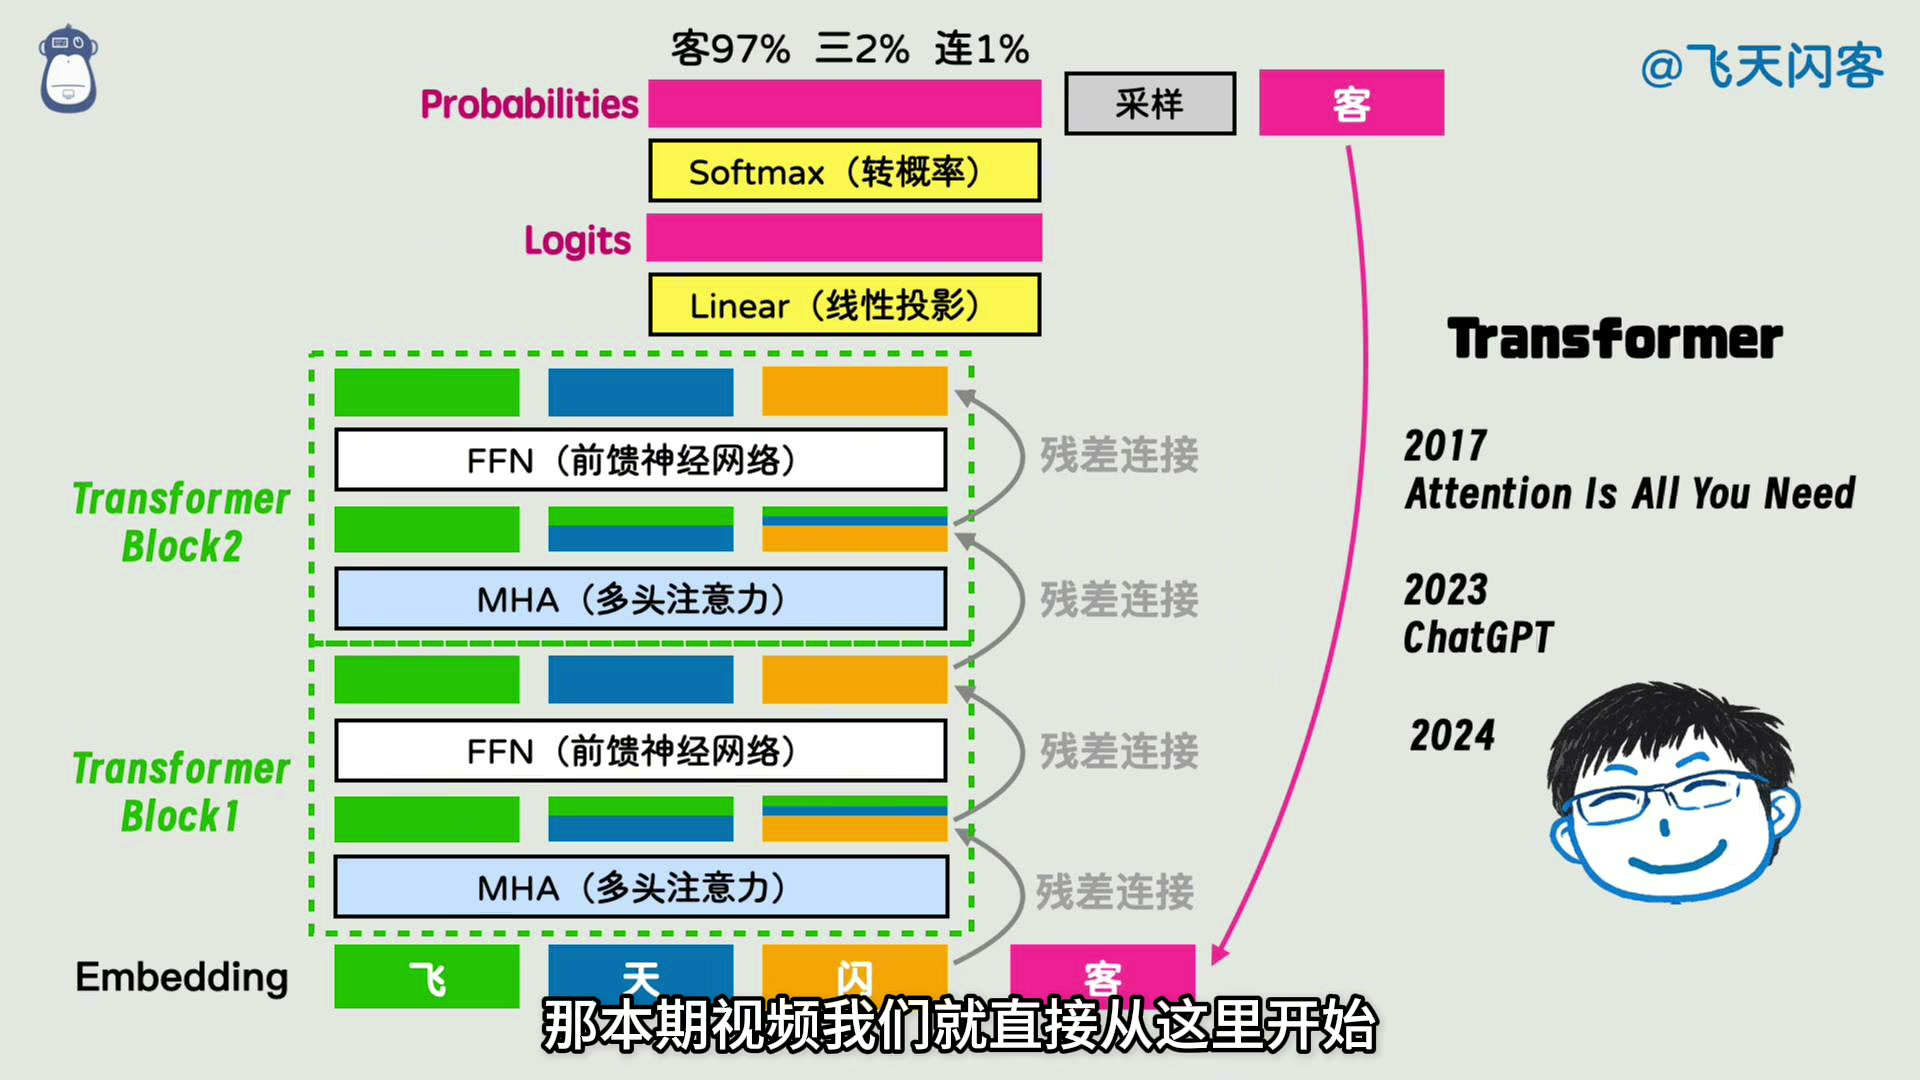
\includegraphics[width=0.6\textwidth]{frame_1.jpg}
\caption{120s:技术演进主线的开场}
\end{figure}

\textbf{V1(DeepSeek LLM, 2024-01)}:先研究\textbf{缩放定律}(scaling law),补全超参数设置对训练的影响(batch size、学习率、数据量、算力),为后续模型规模扩张与超参选择奠定理论基础;并顺手训练出第一个模型 DeepSeek LLM,开启 DeepSeek 的"长期主义"技术路线。

\begin{figure}[h!]
\centering
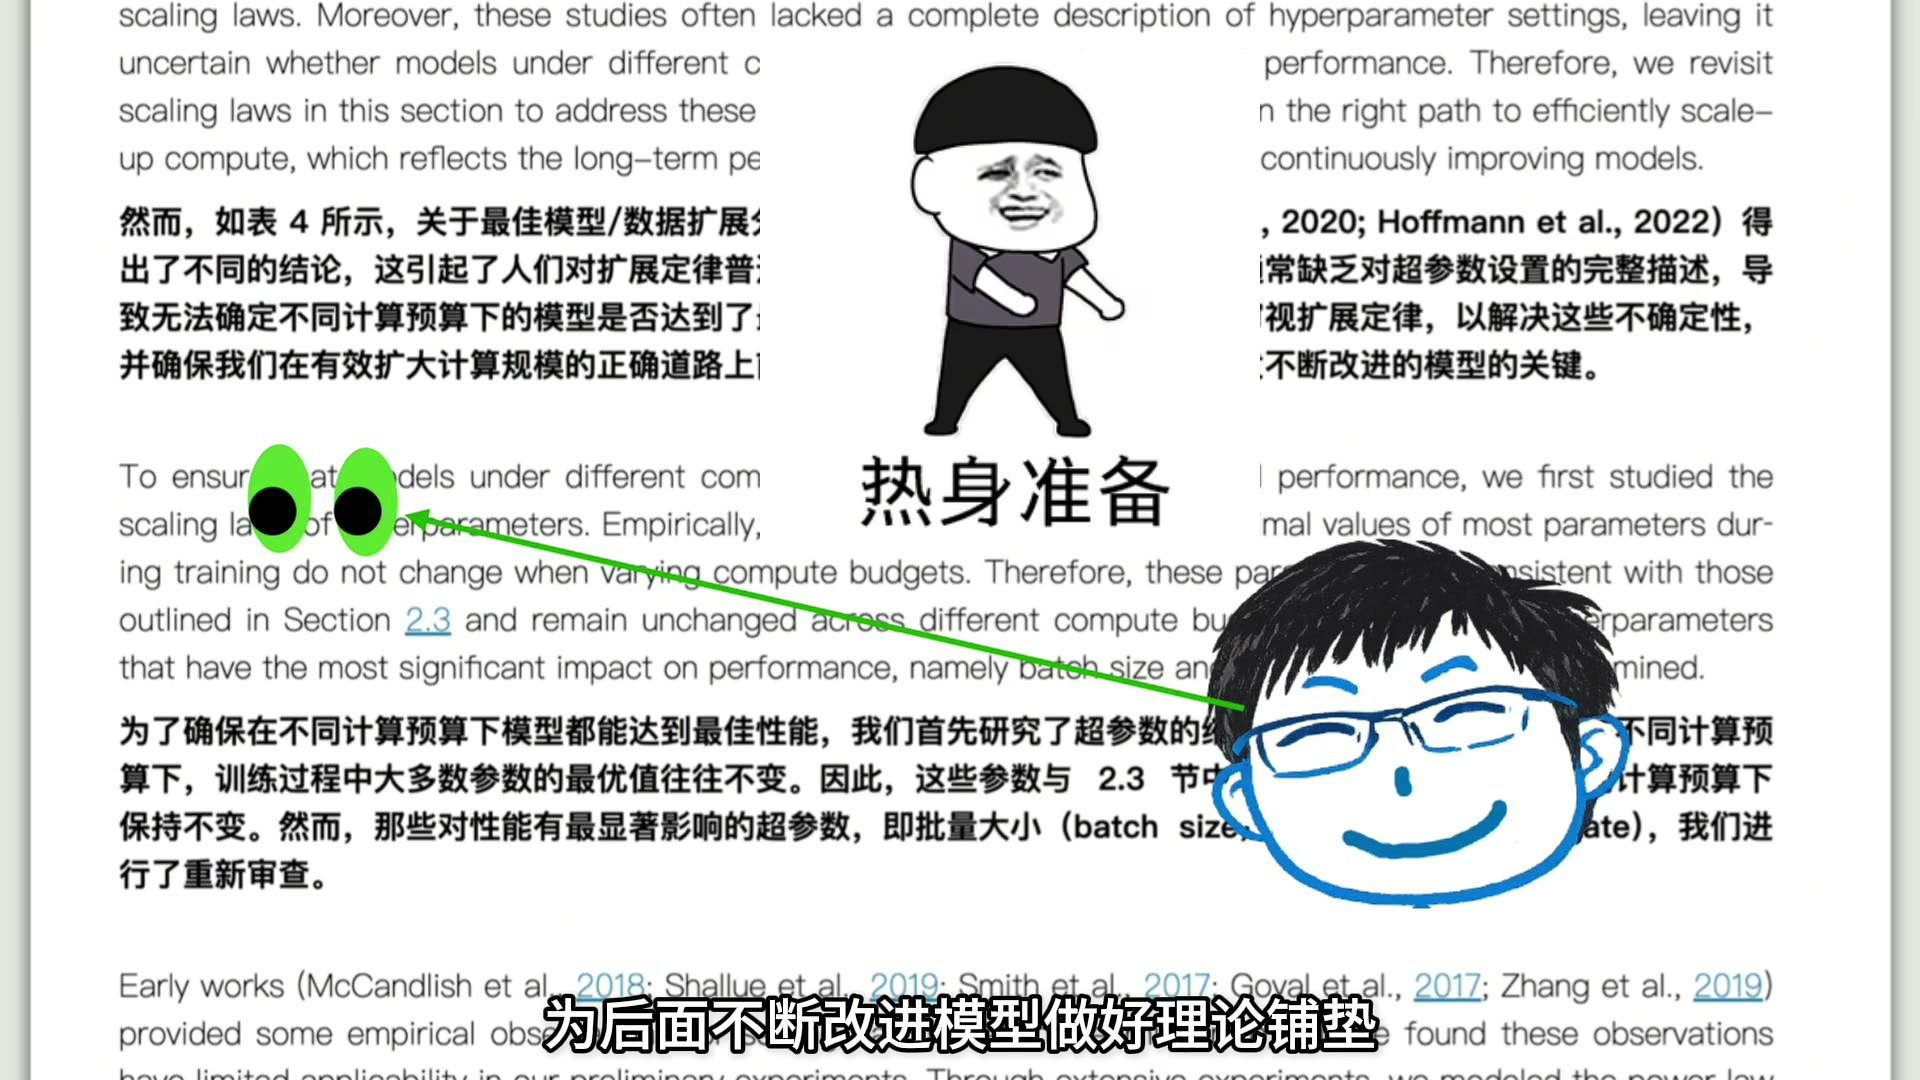
\includegraphics[width=0.6\textwidth]{frame_2.jpg}
\caption{150s:缩放定律研究(超参数对训练的影响)}
\end{figure}

\textbf{V2}:两个关键创新 ——
\begin{itemize}
  \item \textbf{DeepSeekMoE}:FFN 拆成多个专家,每个 token 只路由到部分专家参与计算,总参数量不变但单 token 计算量骤减;关键改良是\textbf{细粒度专家划分}(更多、更小的专家)与\textbf{共享专家}(每个 token 都访问)。
  \item \textbf{MLA(多头潜在注意力)}:认为 KV 向量存在冗余(类似图像可被 VAE 压缩),先把所有 token 的 KV 压缩成一个低维 latent,使用时再还原,大幅降低 KV cache 占用。
\end{itemize}

\begin{figure}[h!]
\centering
\begin{minipage}{0.47\textwidth}
\centering
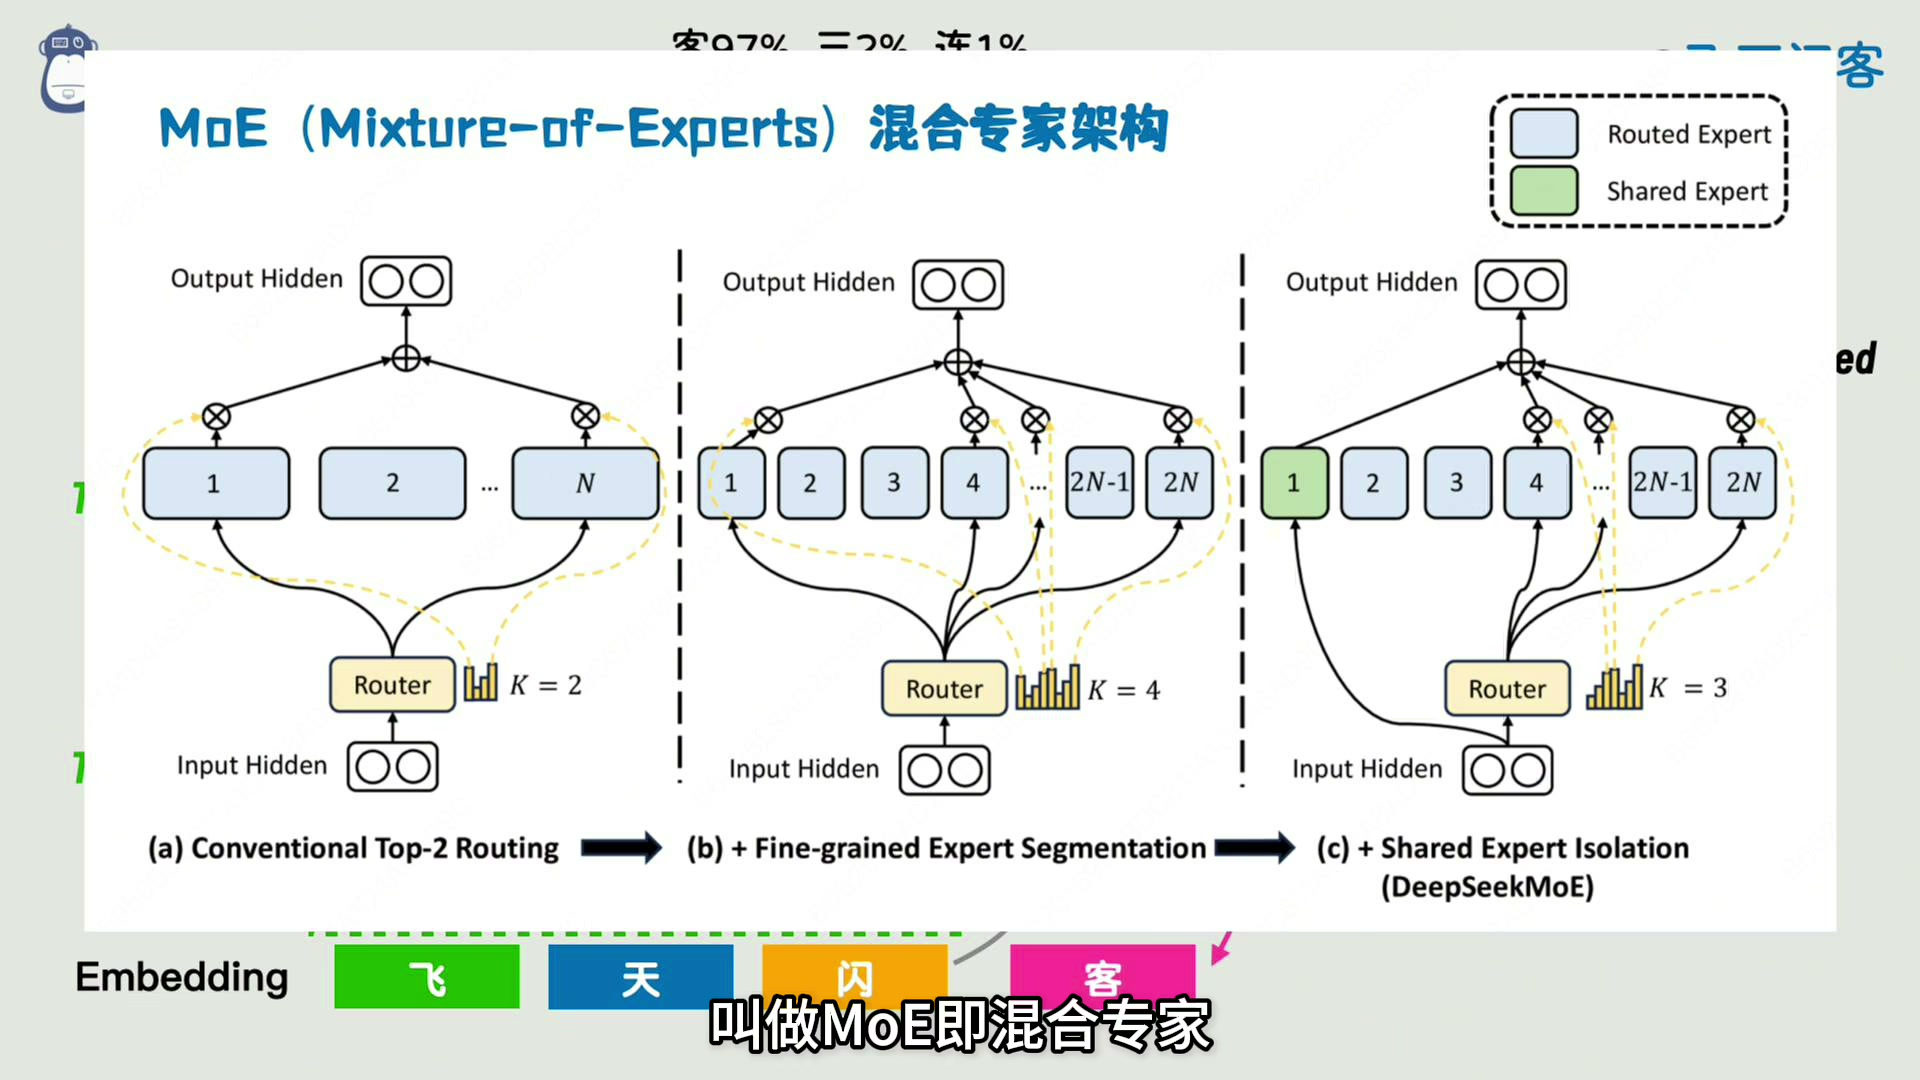
\includegraphics[width=\textwidth]{frame_5.jpg}
\caption{210s:DeepSeekMoE(FFN 拆专家)}
\end{minipage}\hfill
\begin{minipage}{0.47\textwidth}
\centering
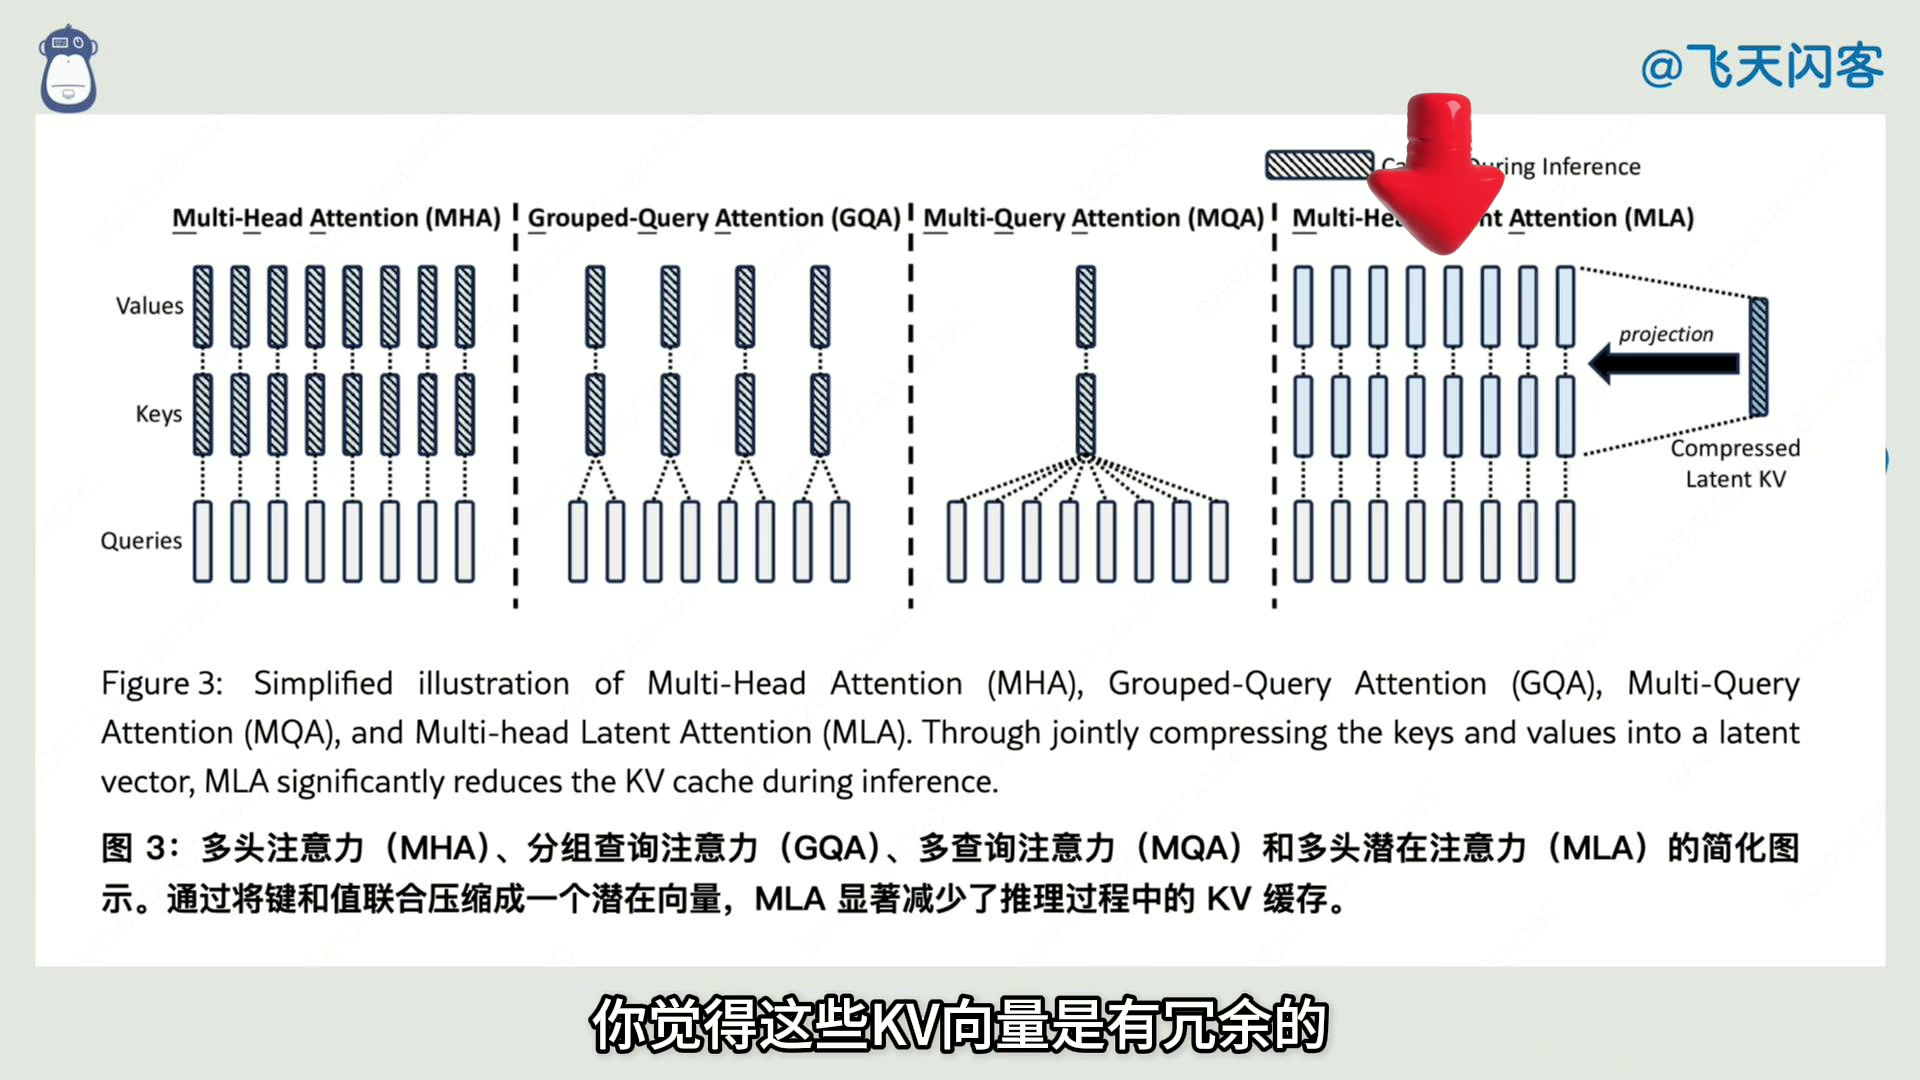
\includegraphics[width=\textwidth]{frame_3.jpg}
\caption{330s:MLA(压缩 KV 为 latent)}
\end{minipage}
\end{figure}

\textbf{V3}:总参数 \textbf{671B MoE、激活仅 37B},综合 MLA、DeepSeekMoE 与多 token 预测(MTP)等工程优化,以极低的训练成本与稳定的训练过程,达到比肩前沿模型的开源性能,从此引爆开源社区关注。

\begin{figure}[h!]
\centering
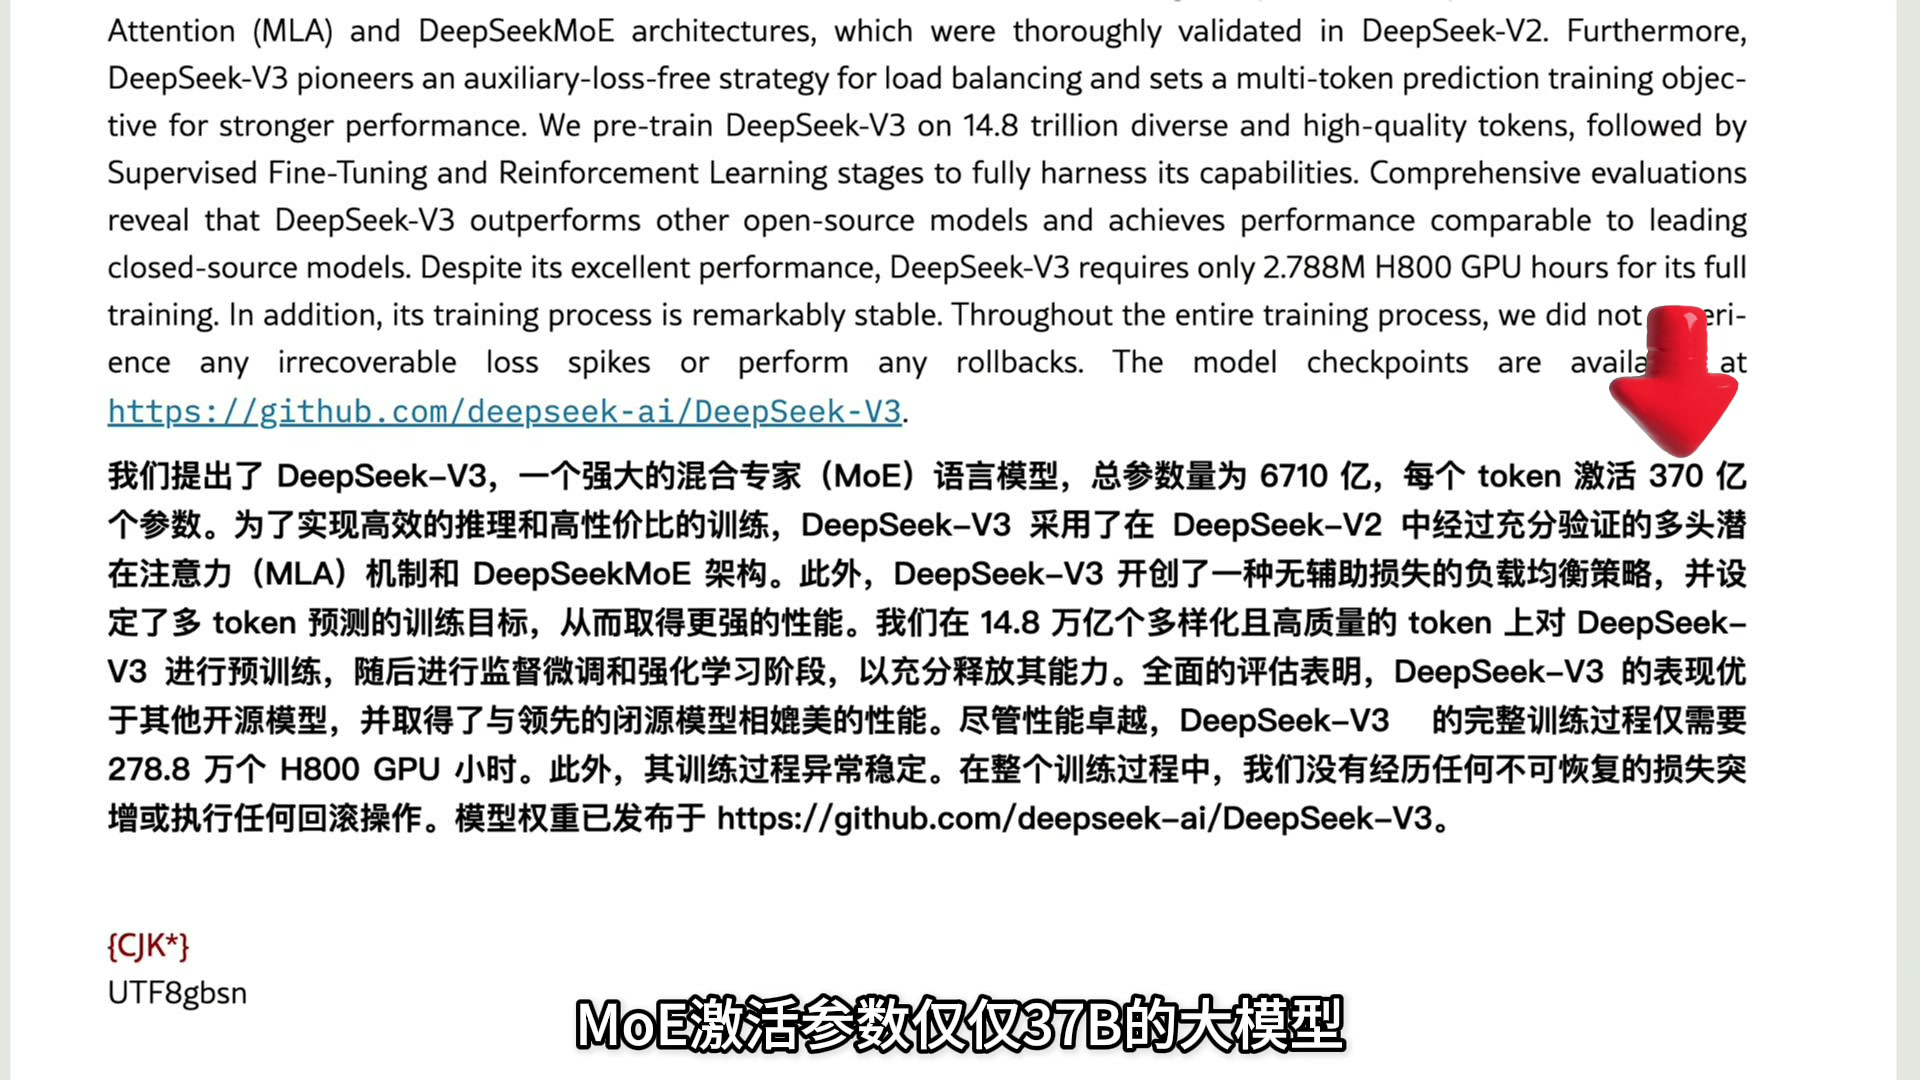
\includegraphics[width=0.6\textwidth]{frame_8.jpg}
\caption{390s:V3 671B / 37B 激活展示}
\end{figure}

\textbf{R1}:做出"违背祖宗的创新"——用\textbf{纯强化学习(GRPO)}训练推理能力,不做传统 SFT:让模型自由发挥,答对奖励、答错惩罚。令人意外的是,模型自发涌现出推理行为,甚至出现 "Aha moment"(输出中途自我纠错、推翻结论),开创了推理模型的新范式。

\begin{figure}[h!]
\centering
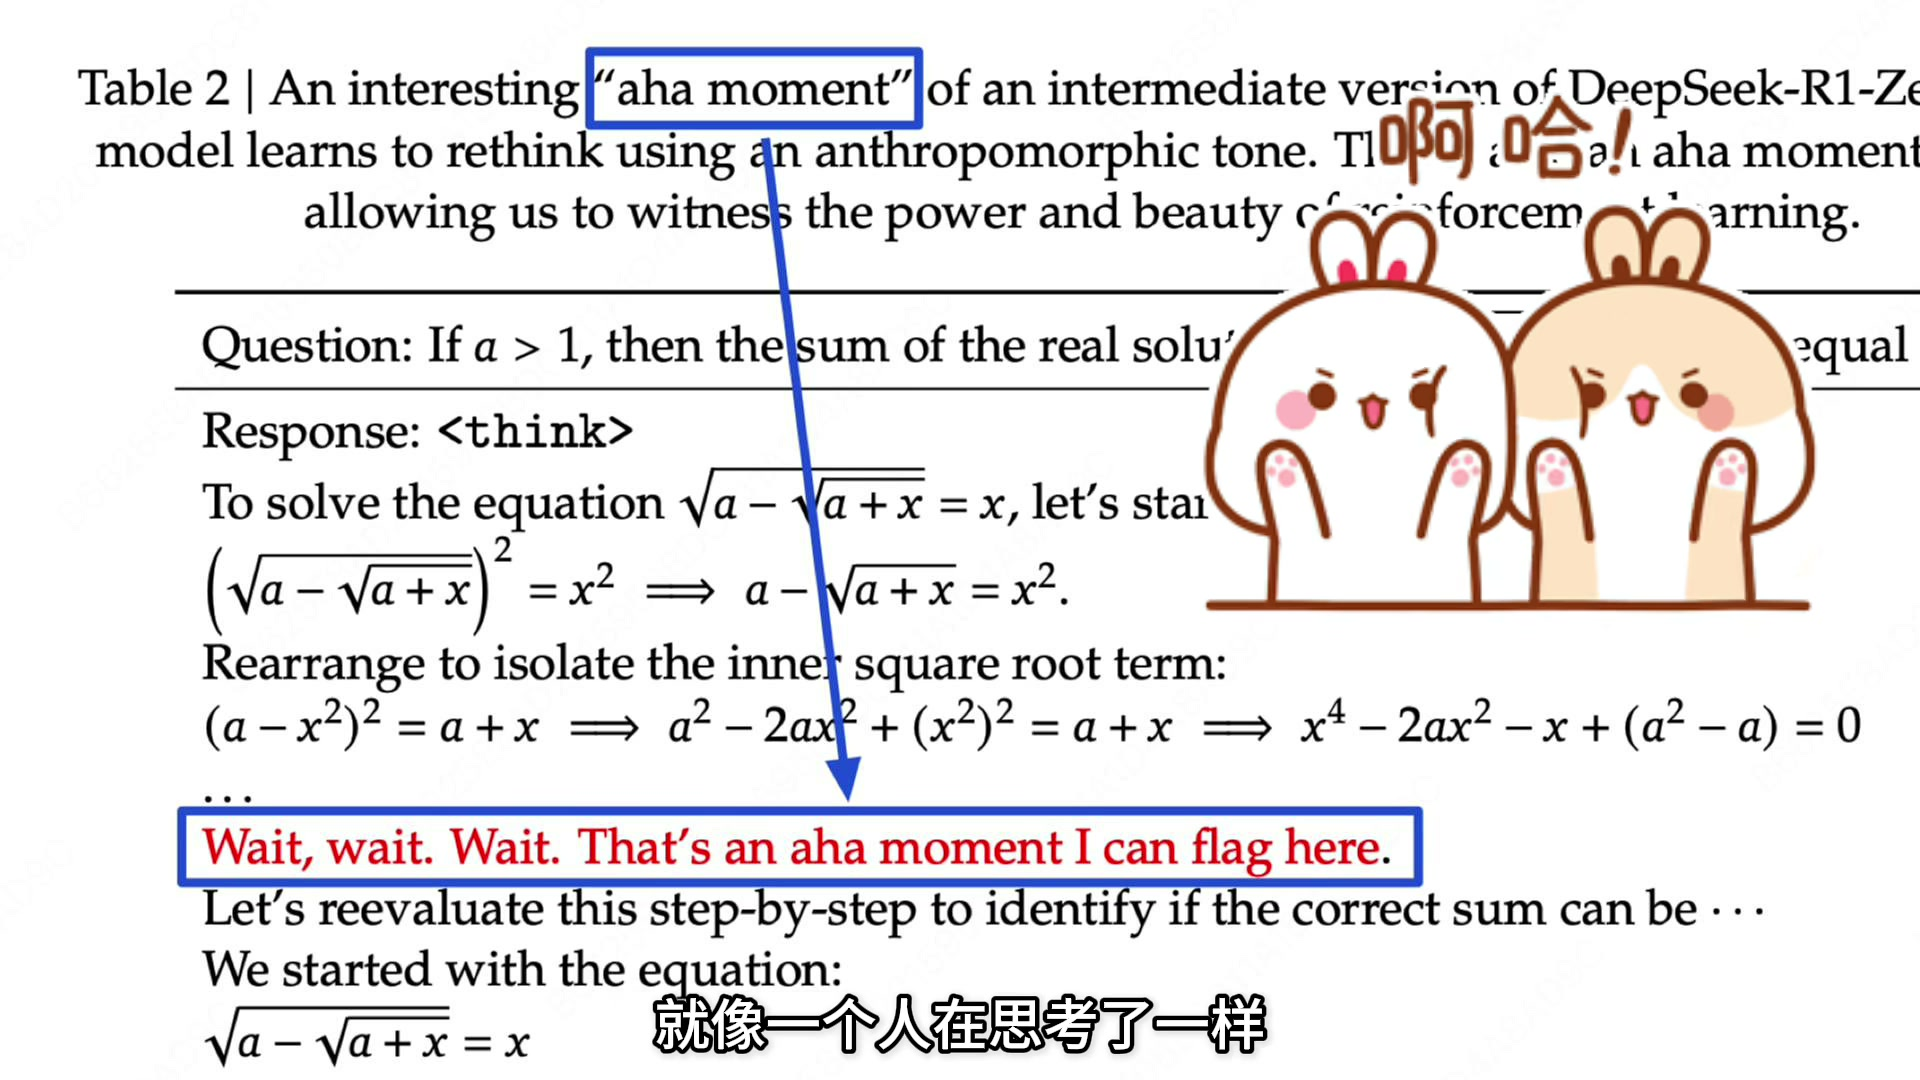
\includegraphics[width=0.6\textwidth]{frame_4.jpg}
\caption{460s:R1 纯强化学习 / Aha moment}
\end{figure}

\textbf{V3.2 / V4}:\textbf{DSA}(DeepSeek 稀疏注意力)通过策略找相关 token,不固定窗口;V4 用 \textbf{CSA + HCA} 混合注意力把长上下文开销压下来。

\begin{note}
\textbf{关键洞见}:V4 的注意力效率不是一步到位。MLA(V2)证明"KV 可压缩",DSA(V3.2)证明"attention 可稀疏",V4 把两者合成 CSA,再加 HCA 做更激进压缩。这正是"来时路的总和"。
\end{note}

\section{三大架构创新}

\subsection{混合注意力:CSA + HCA}

标准注意力对每个 query 都要计算与全部历史 KV 的相关性,复杂度 $O(n^2)$。上下文到百万级后,单 token 推理 FLOPs 与 KV cache 都不可承受。

\begin{definition}{压缩稀疏注意力 CSA}{csa}
两步走:(1) \textbf{压缩 KV}:每 $m$ 个 token 的 KV 压缩成 1 条压缩 KV 条目,序列长度压到 $1/m$;(2) \textbf{稀疏选择}:在压缩 KV 上做 DSA,用 Lightning Indexer 以低秩方式选出 top-$k$ 条最相关条目做核心注意力,另保留小滑动窗口的原始 KV 增强局部依赖。
\end{definition}

\begin{definition}{重度压缩注意力 HCA}{hca}
把每 $m'\gg m$ 个 token 合并成 1 条,压缩更狠,但保持稠密注意力(不再稀疏选择),承担"全局概况"角色。
\end{definition}

CSA 与 HCA 交错布置成混合结构:局部细节由 CSA 的滑动窗口捕捉,长程结构由 HCA 兜底。这是把"稀疏(选谁)"与"压缩(怎么压)"两种思路组合进一个模型。

\textbf{Lightning Indexer}。CSA 的稀疏选择由一个轻量索引器完成:它复用压缩算子生成压缩后的 indexer keys,再以低秩方式(先降维再升维)为每个 query 生成多条 indexer queries,计算与各压缩块的相似度得分,选出 top-$k$ 条参与核心注意力。该 indexer 的 QK 路径在推理与后训练中以 FP4 精度运行,显著加速长上下文下的注意力分数计算。

\begin{figure}[h!]
\centering
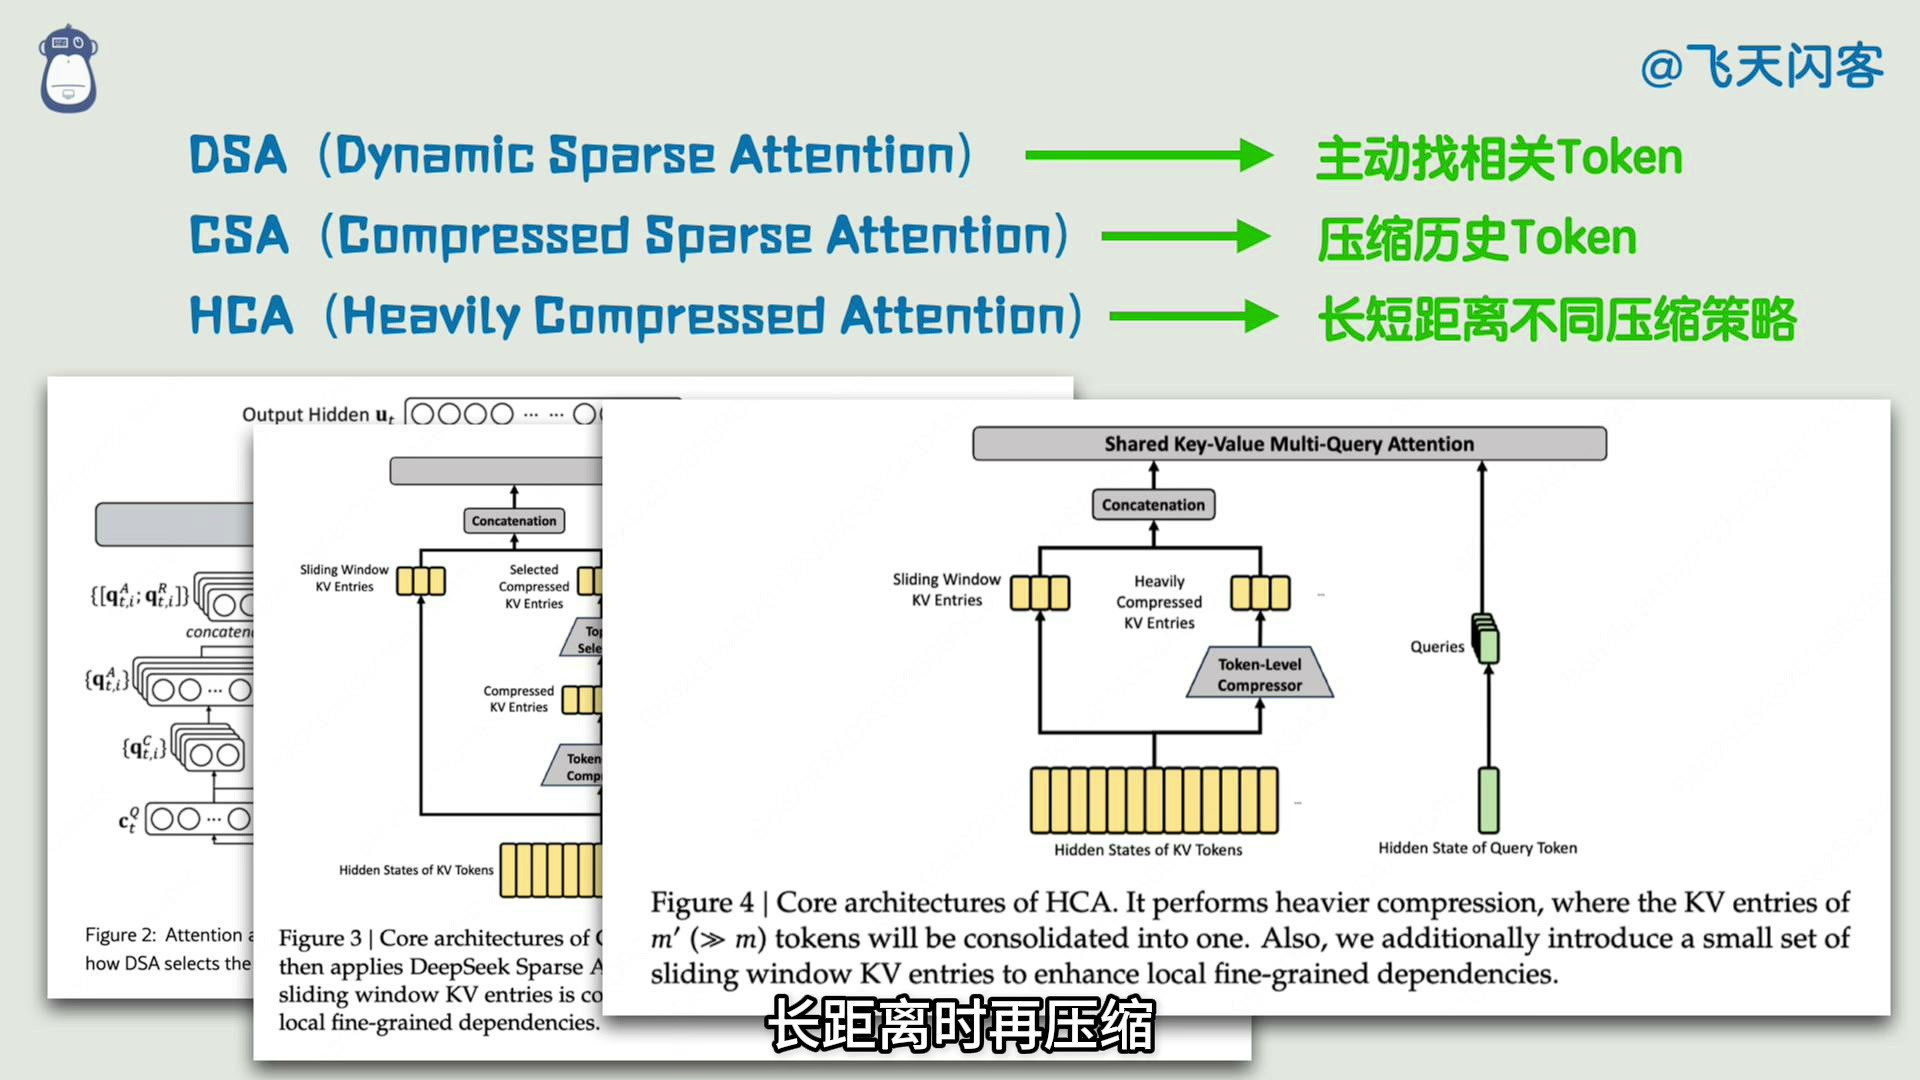
\includegraphics[width=0.6\textwidth]{frame_13.jpg}
\caption{640s:CSA / HCA 注意力压缩讲解}
\end{figure}

\subsection{mHC:流形约束超连接}

\begin{note}
\textbf{问题}:朴素残差连接 $x_{l+1}=x_l+F(x_l)$ 信息传递太死板;HC(字节)把残差流宽度扩到 $n_{hc}\cdot d$,用三个可学习映射 $A,B,C$ 控制信息流,但 $B$ 连乘可能让谱范数失控导致梯度爆炸。
\end{note}

\textbf{mHC 的约束}:把残差映射矩阵 $B$ 投影到\textbf{双随机矩阵流形(Birkhoff 多面体)}
\[
\mathcal{M}\mathrel{:=}\{M\in\mathbb{R}^{n\times n}: M\mathbf{1}_n=\mathbf{1}_n,\ \mathbf{1}_n^\top M=\mathbf{1}_n^\top,\ M\ge 0\}.
\]
约束后谱范数 $\|B\|_2\le 1$,映射非扩张,前向/反向传播数值稳定;该集合对乘法封闭,深层堆叠依然稳定。投影用 \textbf{Sinkhorn-Knopp 迭代}(20 次):先 $\exp$ 保证非负,再交替行/列归一化。$A$、$C$ 映射用 Sigmoid 约束非负有界。

\textbf{动态参数化}。三个映射的参数并非静态,而是由输入动态生成:对残差状态做 RMSNorm 展平后,分别经可学习的低秩投影 $W^{\mathrm{pre}},W^{\mathrm{res}},W^{\mathrm{post}}$ 生成原始参数,再叠加静态偏置,最后经上述约束(投影到双随机流形 / Sigmoid)得到最终映射。这样既保留残差路径的表达力,又保证信号不发散。

\textbf{直觉}:相当于给残差连接装了一个"能量守恒"约束——信息可以重组但不能发散。

\begin{figure}[h!]
\centering
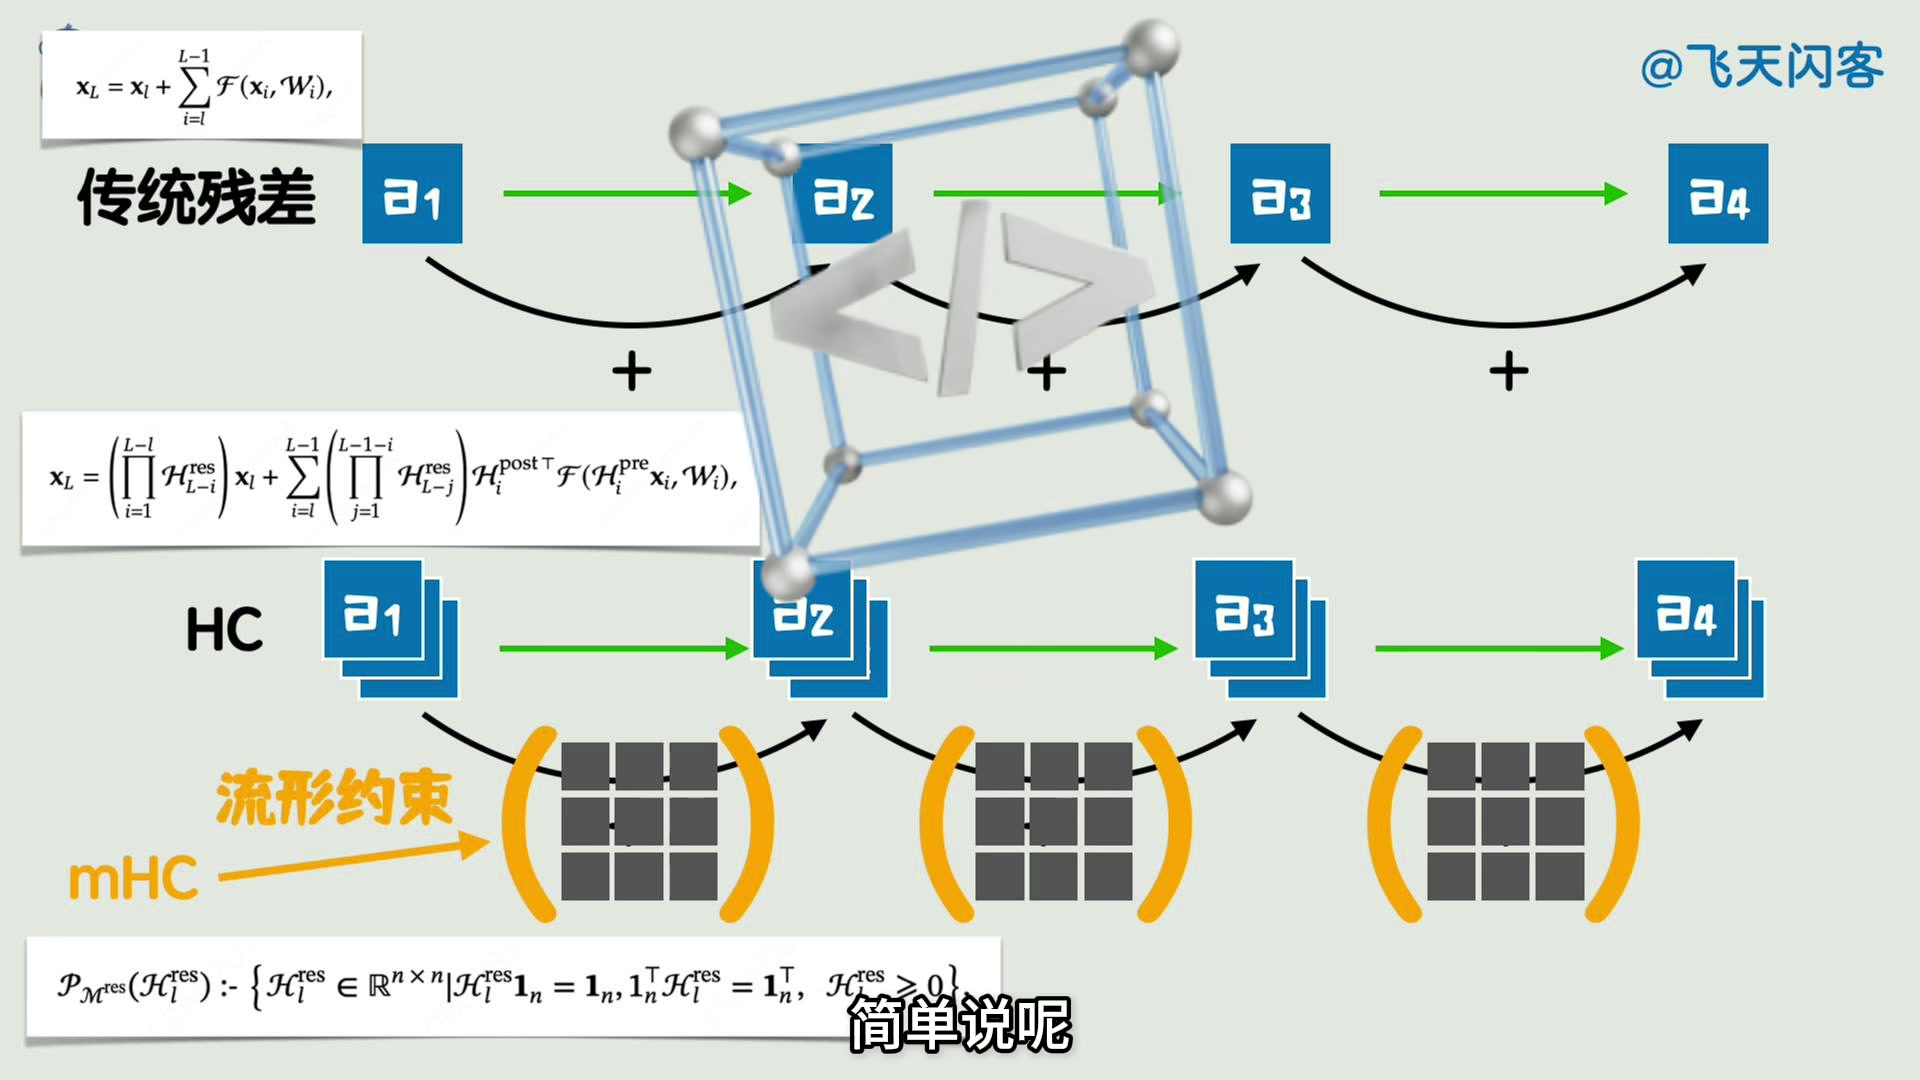
\includegraphics[width=0.6\textwidth]{frame_11.jpg}
\caption{555s:mHC 残差约束讲解}
\end{figure}

\subsection{Muon 优化器}

V3 用 AdamW,V4 的大部分模块换用 \textbf{Muon}——一种矩阵级优化器,通过牛顿-舒尔茨(Newton--Schulz)迭代对参数矩阵做正交化式更新,收敛更快、训练更稳。具体配置:momentum 0.95、weight decay 0.1,并将每步更新矩阵的 RMS 重标至 0.18 以复用 AdamW 学习率。工程上配套 hybrid ZeRO 分片与 BF16 梯度同步(详见 §4.3),保证逐位可复现。

\subsection{其他细节}

除三大创新外,V4 还对 V3 框架做了若干细节调整:MoE 路由亲和度从 Sigmoid 改为 \textbf{Sqrt(Softplus)};去除路由目标节点数约束并重新设计并行策略以维持训练效率;前几个 Transformer block 的稠密 FFN 换成基于 \textbf{Hash routing} 的 MoE(按输入 token ID 的哈希函数确定目标专家,省去路由学习);仍采用 auxiliary-loss-free 负载均衡,并辅以轻量序列级均衡 loss 防止单序列内极端不均衡。

\section{训练与基础设施}

\subsection{预训练:数据、配置与稳定性}

\textbf{数据构建。} 在 DeepSeek-V3 预训练语料之上,V4 构建了更多样、更高质量、上下文更长的训练语料(Flash 32T / Pro 33T tokens)\cite{arxiv}。对网页数据实施过滤策略,剔除批量自动生成与模板化内容以降低模型坍缩风险;数学与编程语料仍为核心,并在中期训练阶段引入 agentic 数据强化编程能力;多语言语料扩大,以覆盖跨文化长尾知识;特别强调长文档语料——科学论文、技术报告等具有学术价值的材料。词表保持 128K,继承 V3 的 token 切分与 Fill-in-Middle(FIM)策略,并改用样本级注意力掩码。

\textbf{模型配置。} 两个模型均采用 CSA/HCA 交错布置,CSA 压缩率 $m{=}4$、HCA 压缩率 $m'{=}128$,滑动窗口大小为 128。表 \ref{tab:modelcfg} 汇总关键结构参数。

\begin{table}[h]
\centering
\caption{V4-Flash 与 V4-Pro 关键结构参数\cite{arxiv}}
\label{tab:modelcfg}
\begin{tabular}{lcc}
\hline
参数 & Flash & Pro \\
\hline
Transformer 层数 & 43 & 61 \\
隐层维度 $d$ & 4096 & 7168 \\
CSA 压缩率 $m$ / HCA $m'$ & 4 / 128 & 4 / 128 \\
稀疏注意 top-$k$ & 512 & 1024 \\
query 头数 & 64 & 128 \\
head 维度 & 512 & 512 \\
query 压缩维度 $d_c$ & 1024 & 1536 \\
输出投影组数 $g$ & 8 & 16 \\
路由专家数(每 token 激活 6) & 256 & 384 \\
专家中间维度 & 2048 & 3072 \\
mHC 扩展因子 $n_{hc}$ / Sinkhorn 迭代 & 4 / 20 & 4 / 20 \\
总参数 / 激活参数 & 284B / 13B & 1.6T / 49B \\
\hline
\end{tabular}
\end{table}

\textbf{训练配置。} 采用混合优化器:大部分参数用 \textbf{Muon}(momentum 0.95、weight decay 0.1,更新矩阵 RMS 重标至 0.18 以复用 AdamW 学习率),embedding、预测头与 RMSNorm 权重用 AdamW($\beta_1{=}0.9,\ \beta_2{=}0.95,\ \varepsilon{=}10^{-20}$)。Flash 最大 batch 75.5M、峰值学习率 $2.7{\times}10^{-4}$;Pro 最大 batch 94.4M、峰值学习率 $2.0{\times}10^{-4}$。两者均采用 2000 步线性 warmup + cosine 衰减,序列长度由 4K 逐步扩展到 16K、64K 直至 1M。注意力稀疏化并非一步到位:前 1T tokens 用稠密注意力预热,在 64K 序列长度时引入稀疏注意力,并对 CSA 的 Lightning indexer 做短阶段预热。

\textbf{训练稳定性。} 万亿参数 MoE 训练极易出现 loss spike;论文将其归因于 MoE 层中的离群值,且路由机制会放大该问题。两项针对性技术:
\begin{itemize}
  \item \textbf{Anticipatory Routing(前瞻路由)}:解耦主干网络与路由网络的同步更新——第 $t$ 步用当前参数计算特征,但路由索引由历史参数 $\theta_{t-\Delta t}$ 提前计算并缓存;配合流水线调度,额外开销仅约 20\%,且仅在自动检测到 loss spike 时触发短回滚启用,随后自动恢复常规训练。
  \item \textbf{SwiGLU Clamping}:将 SwiGLU 的线性分量截断到 $[-10,10]$,gate 分量上界设为 10,在不损失性能的前提下显著抑制离群值。
\end{itemize}

\subsection{后训练:两阶段范式}

与 V3.2 相比,后训练管线最关键的改动是:将混合 RL 阶段整体替换为 \textbf{On-Policy Distillation(OPD)}\cite{arxiv}。

\textbf{阶段一:领域专家训练。} 对数学、代码、Agent、指令遵循等领域分别执行 SFT + 领域 GRPO,得到专业专家。要点包括:
\begin{itemize}
  \item \textbf{三档推理模式}:Non-think / Think High / Think Max,由 \texttt{<think>} 标记配合不同的长度惩罚与上下文窗口实现;Think Max 模式在 system prompt 注入"最大推理强度、禁止捷径"等指令。
  \item \textbf{生成式奖励模型(GRM)}:对难验证任务不使用标量奖励模型,而是让 actor 网络原生充当 GRM,将评判与生成能力联合优化,仅需少量多样化人类标注。
  \item \textbf{工具调用 schema}:以 \texttt{|DSML|} 特殊 token + XML 格式调用工具,有效减少转义失败与工具调用错误。
  \item \textbf{交错的思考(Interleaved Thinking)}:工具调用场景中,借助 1M 上下文保留全部推理历史(跨用户消息也不丢弃),维持长程 Agent 任务的连贯推理;普通对话场景则仍丢弃旧推理以保持上下文精简。
  \item \textbf{Quick Instruction}:在输入序列追加专用特殊 token(如是否触发搜索、生成标题/query、判断权威性),直接复用已计算的 KV cache,避免冗余 prefill,显著降低首 token 延迟(TTFT)。
\end{itemize}

\textbf{阶段二:多教师 on-policy 蒸馏。} 训练统一 student 模型,对 10 余个领域专家教师优化反向 KL 散度(式 \ref{eq:opd});学生用自己的轨迹采样,保证 on-policy。与常见的逐 token KL 估计相比,V4 采用\textbf{全词表 logit 蒸馏},梯度估计更稳定、保真度更高。

\begin{equation}
\label{eq:opd}
\mathcal{L}_{\mathrm{OPD}}(\theta)=\sum_{i=1}^{N} w_i\, D_{\mathrm{KL}}\bigl(\pi_\theta \parallel \pi_{E_i}\bigr).
\end{equation}

这一"分而治之再蒸馏"的范式,使 1.6T 参数的通用模型能够在数学、代码、Agent 等多个领域同时保持强性能——而非单一 SFT 阶段的数据堆叠。

\subsection{基础设施}

\textbf{细粒度专家并行(EP)。} MoE 层可分解为 Dispatch(通信)、Linear-1(计算)、Linear-2(计算)、Combine(通信)四个阶段,且单层内通信总时长小于计算时长。V4 将专家按 wave 切分调度,形成计算、下一波 token 传输、已完成波结果回传三者并发的细粒度流水线(理论加速 1.92$\times$),在 NVIDIA GPU 与华为昇腾 NPU 上实测通用推理加速 1.50--1.73$\times$,RL rollout 等延迟敏感场景最高 1.96$\times$;CUDA mega-kernel 已以 \texttt{MegaMoE} 开源并入 DeepGEMM。论文据此给出硬件建议:计算/通信比达 $C/B\le 2d{=}6144$ FLOPs/Byte 后,带宽不再是瓶颈,再增带宽收益递减。

\textbf{TileLang DSL。} 用领域专用语言 TileLang 开发融合 kernel,替代数百个 Torch ATen 算子。关键工程:① Host Codegen 将运行期校验移出 Python 执行路径,单次调用校验开销从数百微秒降至 $<1\mu s$;② 集成 Z3 SMT 求解器做形式化整数分析(布局推断、内存冲突、边界分析),以数秒级编译开销提升向量化等优化能力;③ 默认关闭 fast-math、对齐 CUDA 工具链,实现位级(bitwise)可复现。

\textbf{Batch-invariant 确定性 kernel。} 为保证任意 token 的输出与其在 batch 中的位置无关(跨预训练/后训练/推理逐位对齐),注意力解码采用双 kernel 策略规避 wave-quantization;矩阵乘全线替换为 DeepGEMM 并弃用 split-k。反传确定性:注意力反传为每个 SM 分配独立累加缓冲再做全局确定性求和,MoE 反传做 token 排序预处理与跨 rank 缓冲隔离,mHC 的小矩阵反传先输出各 split 再确定性归约。

\textbf{训练框架。}
\begin{itemize}
  \item \textbf{Muon 高效实现}:Muon 需要完整梯度矩阵,与传统 ZeRO 参数分区冲突;V4 采用混合 ZeRO bucket 分配——稠密参数用背包算法均衡分配并限制并行度,MoE 参数按专家独立展平分发;连续同形状参数合并以批量执行 Newton--Schulz 迭代;利用 BF16 下 Newton--Schulz 仍稳定的性质,以随机舍入将 MoE 梯度同步压缩到 BF16,通信量减半。
  \item \textbf{mHC 节省实现}:融合 kernel + 选择性重算(重算层间隐状态与归一化输入,但避免重算计算密集操作)+ 调整 DualPipe 1F1B 重叠,使 mHC 的 wall-time 开销仅占重叠流水线阶段的 6.7\%。
  \item \textbf{上下文并行(CP)}:针对压缩注意力的两阶段通信——先由每个 rank 把尾部 $m$ 条未压缩 KV 传给下一 rank 完成跨边界压缩,再 all-gather 全部压缩 KV,由 fused select-and-pad 重组。
  \item \textbf{张量级激活检查点}:基于 TorchFX 追踪计算图,开发者只需注解张量,框架自动回溯出最小重算子图并插入反传;重算通过释放显存并复用指针实现,零拷贝、零额外训练开销。
\end{itemize}

\textbf{推理框架:异构 KV cache 与磁盘存储。} 混合注意力产生多种大小与更新规则各异的 KV 条目,无法直接套用 PagedAttention 的假设。V4 将 KV cache 分为两部分:经典 KV cache(CSA/HCA 压缩 KV)与 \textbf{state cache}(滑动窗口注意力与未压缩尾部 token);每个请求分配定长缓存块,块长按 $m$、$m'$ 的最小公倍数对齐。共享前缀请求通过磁盘 KV 存储消除重复 prefill:CSA/HCA 压缩 KV 直接落盘复用;SWA KV 体积约为压缩 KV 的 8 倍,提供\textbf{全量缓存 / 周期检查点 / 零缓存重算}三种策略,权衡存储与计算开销。

\textbf{后训练基建。}
\begin{itemize}
  \item \textbf{FP4 量化感知训练(QAT)}:对 MoE 专家权重与 CSA indexer 的 QK 路径做 FP4 量化,index 分数由 FP32 降至 BF16;top-k 选择器加速 2$\times$ 且保持 99.7\% 的 KV 召回率。FP4$\to$FP8 反量化无损(FP8 的 E4M3 比 FP4 的 E2M1 多 2 个指数位)。
  \item \textbf{全词表 OPD 教师调度}:教师权重经分布式存储按需加载(ZeRO 式分片),仅缓存教师最后一层隐状态、训练时实时重建全词表 logits,避免 $|V|>100k$ 的 logits 显式落盘;按教师索引排序样本,保证每个 mini-batch 至多一个教师头驻留显存。
  \item \textbf{可抢占容错 rollout}:token 粒度 Write-Ahead Log(WAL) + 抢占时保存 KV cache,恢复时无缝续解码;硬件故障时用 WAL 重跑 prefill 即可重建 KV cache,避免从零重生成引入的长度偏差。
  \item \textbf{百万上下文 RL}:rollout 数据拆分为轻量元数据与重 per-token 字段,经共享内存加载器按 mini-batch 消费,大幅降低 CPU/GPU 内存压力。
  \item \textbf{Agent 沙箱(DSec)}:基于 3FS 的弹性计算平台,单集群可管理数十万并发沙箱;以统一 Python SDK 抽象函数调用、容器、microVM、fullVM 四类执行基座,支持分层按需镜像加载与轨迹日志驱动的确定性重放。
\end{itemize}

\section{效率与评测数据}

\begin{table}[h]
\centering
\caption{1M token 上下文下的效率(相对 DeepSeek-V3.2)}
\begin{tabular}{lcc}
\hline
模型 & 单 token 推理 FLOPs & KV cache \\
\hline
DeepSeek-V4-Pro   & $27\%$ & $10\%$ \\
DeepSeek-V4-Flash & $10\%$ & $7\%$  \\
\hline
\end{tabular}
\end{table}

注:FP4$\times$FP8 在当前硬件峰值 FLOPs 与 FP8$\times$FP8 相同,但未来硬件理论上可再省 $1/3$ 算力。

\begin{table}[h]
\centering
\caption{评测要点(V4-Pro-Max)}
\begin{tabular}{lp{9.5cm}}
\hline
维度 & 表现 \\
\hline
知识 & SimpleQA / 中文 SimpleQA 显著领先开源;MMLU-Pro / HLE / GPQA 小幅领先开源,紧追 Gemini-3.1-Pro \\
推理 & 强于 GPT-5.2、Gemini-3.0-Pro;弱于 GPT-5.4、Gemini-3.1-Pro,落后前沿约 3--6 个月 \\
Agent & 与 Kimi-K2.6、GLM-5.1 持平;内部评测优于 Claude Sonnet 4.5,接近 Opus 4.5 \\
长上下文 & 1M 上下文学术基准超过 Gemini-3.1-Pro \\
\hline
\end{tabular}
\end{table}

基础模型层面,V4-Flash-Base 以更小的激活/总参数在多数基准上全面超越 V3.2-Base(尤其世界知识与长上下文);V4-Pro-Base 则在几乎所有类别上进一步拉开差距。表 \ref{tab:baseeval} 摘录部分基准。

\begin{table}[h]
\centering
\caption{基础模型评测对比(部分基准)\cite{arxiv}}
\label{tab:baseeval}
\begin{tabular}{lccc}
\hline
基准 & V3.2-Base & V4-Flash-Base & V4-Pro-Base \\
\hline
MMLU (5-shot) & 87.8 & 88.7 & 90.1 \\
MMLU-Pro (5-shot) & 65.5 & 68.3 & 73.5 \\
C-Eval (5-shot) & 90.4 & 92.1 & 93.1 \\
SimpleQA-verified (25-shot) & 28.3 & 30.1 & 55.2 \\
SuperGPQA (5-shot) & 45.0 & 46.5 & 53.9 \\
FACTS Parametric (25-shot) & 27.1 & 33.9 & 62.6 \\
HumanEval (Pass@1) & 62.8 & 69.5 & 76.8 \\
LongBench-V2 (1-shot) & 40.2 & 44.7 & 51.5 \\
\hline
\end{tabular}
\end{table}

值得注意的是,\textbf{SimpleQA-verified} 与 \textbf{FACTS Parametric} 上 V4-Pro-Base 相对 V3.2-Base 近乎翻倍($28.3\to55.2$、$27.1\to62.6$),反映知识密集与事实性任务上的显著增益。

V4-Flash-Max 因参数规模较小,在知识类评测中表现偏弱;但在分配更大的推理预算(thinking budget)时,其推理任务表现可与 Pro-Max 相当\cite{arxiv}。

\section{技术评注}

\begin{enumerate}
  \item \textbf{方向转变:从"堆算力"到"减算力"。} 2026 年的开源竞争早已不是单点参数竞赛。V4 的卖点是百万上下文下的单位算力性价比,与 test-time scaling 趋势契合——上下文越长,注意力开销越占主导,压住它即解锁更长推理。
  \item \textbf{MLA $\to$ CSA 一脉相承。} V2 的 MLA 压缩"每个头的 KV",V4 的 CSA 压缩"序列维度上的 token"。同一信念——KV 存在冗余——在不同维度兑现。
  \item \textbf{mHC 是训练稳定化的隐性功臣。} 它不直接提精度,而是让 1.6T 模型训得动。双随机约束(非扩张映射)是优雅的数学解法。
  \item \textbf{落后前沿 3--6 个月是论文亲口承认的。} 官方技术报告少见地坦诚;DeepSeek 的差异化仍在"效率 + 开源 + 价格"。
  \item \textbf{OPD 替代混合 RL 是一次"收敛性"选择。} 多专家合并若用权重混合或混合 RL,通常伴随性能回退;OPD 用学生自采样的 on-policy 轨迹做全词表 reverse-KL 蒸馏,把物理上分离的专家知识收编到统一参数空间,工程代价由全词表教师调度(§4.3)摊平。
  \item \textbf{1M 上下文的真正意义是解锁 test-time scaling。} 推理模型性能由"推理预算"决定;上下文越长、推理步数越多,注意力开销越占主导。V4 把百万上下文做到可常规部署,等价于把"长时间思考 / 长程工具调用"的成本降下来——这是下一代推理范式的基础设施。
\end{enumerate}

\begin{thebibliography}{9}
\bibitem{arxiv} DeepSeek-AI. \textit{DeepSeek-V4: Towards Highly Efficient Million-Token Context Intelligence}[EB/OL]. arXiv:2606.19348, 2026. \url{https://arxiv.org/abs/2606.19348}.
\bibitem{report} DeepSeek-AI. \textit{DeepSeek-V4 Technical Report}[EB/OL]. Hugging Face, 2026. \url{https://huggingface.co/deepseek-ai/DeepSeek-V4-Pro/blob/main/DeepSeek_V4.pdf}.
\bibitem{wechat} DeepSeek-AI. \textit{DeepSeek-V4 发布公告}[EB/OL]. 微信公众号, 2026. \url{https://mp.weixin.qq.com/s/8bxXqS2R8Fx5-1TLDBiEDg}(抓取时触发微信安全验证,未能直接读取正文).
\bibitem{hf} DeepSeek-AI. \textit{DeepSeek-V4 Models}[EB/OL]. Hugging Face Collection. \url{https://huggingface.co/collections/deepseek-ai/deepseek-v4}.
\bibitem{ms} DeepSeek-AI. \textit{DeepSeek-V4 模型集合}[EB/OL]. ModelScope. \url{https://modelscope.cn/collections/deepseek-ai/DeepSeek-V4}.
\bibitem{video} 闪客. \textit{深入解读 DeepSeek V1~V4!男女老少都听得懂}[EB/OL]. Bilibili, 2026. \url{https://www.bilibili.com/video/BV1rpovBCEGH/}.
\end{thebibliography}

\end{document}
